\documentclass[conference]{IEEEtran}
\IEEEoverridecommandlockouts
\usepackage{cite}
\usepackage{amsmath,amssymb,amsfonts}
\usepackage{algorithmic}
\usepackage{graphicx}
\usepackage{textcomp}
\usepackage{xcolor}
\usepackage{listings}
\usepackage{pgfplots}
\usepackage[bookmarks=true,breaklinks=true,letterpaper=true,colorlinks,linkcolor=black,citecolor=blue,urlcolor=black]{hyperref}

% dsm: Copied from /usr/share/texlive/texmf-dist/tex/latex/listings/lstlang1.sty ,
% but removing bin from morekeywords[2], b/c deletekeywords ignores it somehow.
\lstdefinelanguage{PythonNoBin}%
  {morekeywords={access,and,break,class,continue,def,del,elif,else,%
      except,exec,finally,for,from,global,if,import,in,is,lambda,not,%
      or,pass,print,raise,return,try,while},%
  % Built-ins
   morekeywords=[2]{abs,all,any,basestring,bool,bytearray,callable,chr,
     classmethod,cmp,compile,complex,delattr,dict,dir,divmod,enumerate,eval,
     execfile,file,filter,float,format,frozenset,getattr,globals,hasattr,
     help,hex,id,input,int,isinstance,issubclass,iter,len,list,locals,long,map,
     max,memoryview,min,object,oct,open,ord,pow,property,range,raw_input,
     reduce,reload,repr,reversed,round,set,setattr,slice,sorted,staticmethod,str,
     sum,super,tuple,type,unichr,unicode,vars,xrange,zip,apply,buffer,coerce,
     intern},
   sensitive=true,%
   morecomment=[l]\#,%
   morestring=[b]',%
   morestring=[b]",%
   morestring=[s]{'''}{'''},% used for documentation text (mulitiline strings)
   morestring=[s]{"""}{"""},% added by Philipp Matthias Hahn
   morestring=[s]{r'}{'},% `raw' strings
   morestring=[s]{r"}{"},%
   morestring=[s]{r'''}{'''},%
   morestring=[s]{r"""}{"""},%
   morestring=[s]{u'}{'},% unicode strings
   morestring=[s]{u"}{"},%
   morestring=[s]{u'''}{'''},%
   morestring=[s]{u"""}{"""}%
  }%

  \lstdefinestyle{custompython}{
 %aboveskip=0in,
 belowskip=0in,
 %abovecaptionskip=0in,
 belowcaptionskip=-10pt,
 %belowcaptionskip=1\baselineskip,
 breaklines=true,
 captionpos=b,
 language=PythonNoBin,
 showstringspaces=false,
 numbers=left,
 stepnumber=1,
 % dsm: semibold
 % yyf: semibold will just be bold on Ubuntu 20.04, disable it
 %basicstyle={\linespread{0.75}\fontseries{sb}\small\ttfamily},
 basicstyle={\linespread{0.75}\footnotesize\ttfamily},
 keywordstyle=\bfseries,
 %% columns=fullflexible,
 xleftmargin=2em,
 frame=single,
 framexleftmargin=2em,
 commentstyle=\itshape\color{green!40!black},
 morekeywords={to,yield,parallel},
}


%\def\BibTeX{{\rm B\kern-.05em{\sc i\kern-.025em b}\kern-.08em
%    T\kern-.1667em\lower.7ex\hbox{E}\kern-.125emX}}
\begin{document}

\title{Optimizing a Tensor Product using Sparsity}

\author{\IEEEauthorblockN{Jaeyeon Won}
\and
\IEEEauthorblockN{Ryan Lee}
\and
\IEEEauthorblockN{Nicholas Dow}
}

\maketitle

\begin{abstract}
We present an optimized GPU implementation of the tensor product for equivariant neural networks. Tensor products in equivariant neural networks are challenging due to the block sparsity in its weights imposed by the three properties of equivariance (translation, rotations, and inversion). We show that using the right sparse tensor format is critical to performing only the effectual computations while minimizing costly synchronization between SMs. We implement a GPU implementation using Triton which outperforms the dense Jax-based baseline by XXX$\times$ on a Nvidia RTX A4000 GPU.

\end{abstract}

\section{Introduction}
\label{sec:intro}

INTRO


\section{Background}
\label{sec:background}


\section{Implementation}
\label{sec:impl}

\subsection{Using Coordinate List (COO) Representation}
\label{sec:impl:coo}

The relatively high sparsity of equivariant neural networks guides us to use a \textit{sparse representation} of the weights. Sparse representations such as Coordinate List (COO) and Compressed-Sparse Row only store non-zero values and their coordinates,
which brings the benefit of skipping ineffectual computation (e.g., multiplying by zero). We use the COO format which stores the coordinates of non-zero values as a list of tuples.

%\begin{figure}[!htb]
\begin{lstlisting}[caption={Hash table lookup code.}, label={lst:simple_tensor_prod}, style=custompython]
# B : Batch size
# NNZ: Number of nonzeros
# W_i, W_j, W_k, W_val: weights in COO-format,  dimensions [NNZ]
# Input1, Input2: [B, L_in]
# Output: [B, L_out]
def TensorProduct(W_i, W_j, W_k, W_val, 
  Input1, Input2, Output):
    for nz in range(NNZ):
      nz_in1 = Input1[:,W_i[nz]]
      nz_in2 = Input2[:,W_j[nz]]
      Output[:,W_k[nz]] += nz_in1 * nz_in2 * W_val[nz]
\end{lstlisting}
%\end{figure}

The tensor product kernel is implemented using Triton~\cite{tillet2019triton}.
We design the kernel such that each Triton program works on a \textit{block of non-zeros}.
The pseudocode is given in \autoref{lst:simple_tensor_prod}.
Given the input \texttt{i}, \texttt{j}, and \texttt{k} coordinate values of the COO,
each Triton program loads a block of these coordinates,
performs an indirect load on the input tensors to grab the corresponding values
(\texttt{i} coordinates from the first tensor and \texttt{j} coordinates from the second tensor),
and multiplies them with the weight.
The kernel then performs scatter indirect stores to the \texttt{k} coordinates
of the output tensor.

Our tensor kernel's performance is highly dependent on the number of gather loads of the input tensors
and the scatter writes to the output tensor.
In particular, the scatter writes must be performed \textit{atomically} because different triton programs (i.e., thread blocks in CUDA-land) can write to the same coordinate of the output tensor.
As we will see later in \autoref{sec:eval}, the atomic add operations dominate our throughput such that the naive implementation is worse than the dense baseline.

\subsection{Reducing Atomic Operations}
\label{sec:impl:block}

We reduce the number of atomic operations by \textit{grouping multiple input coordinates that contribute to the same output coordinate}.
Our key insight is that multiple input coordinates that contribute to the same output coordinate can be handled by a single thread,
which removes the need for atomic operations on those FMAs.

\begin{figure}
  \centering
  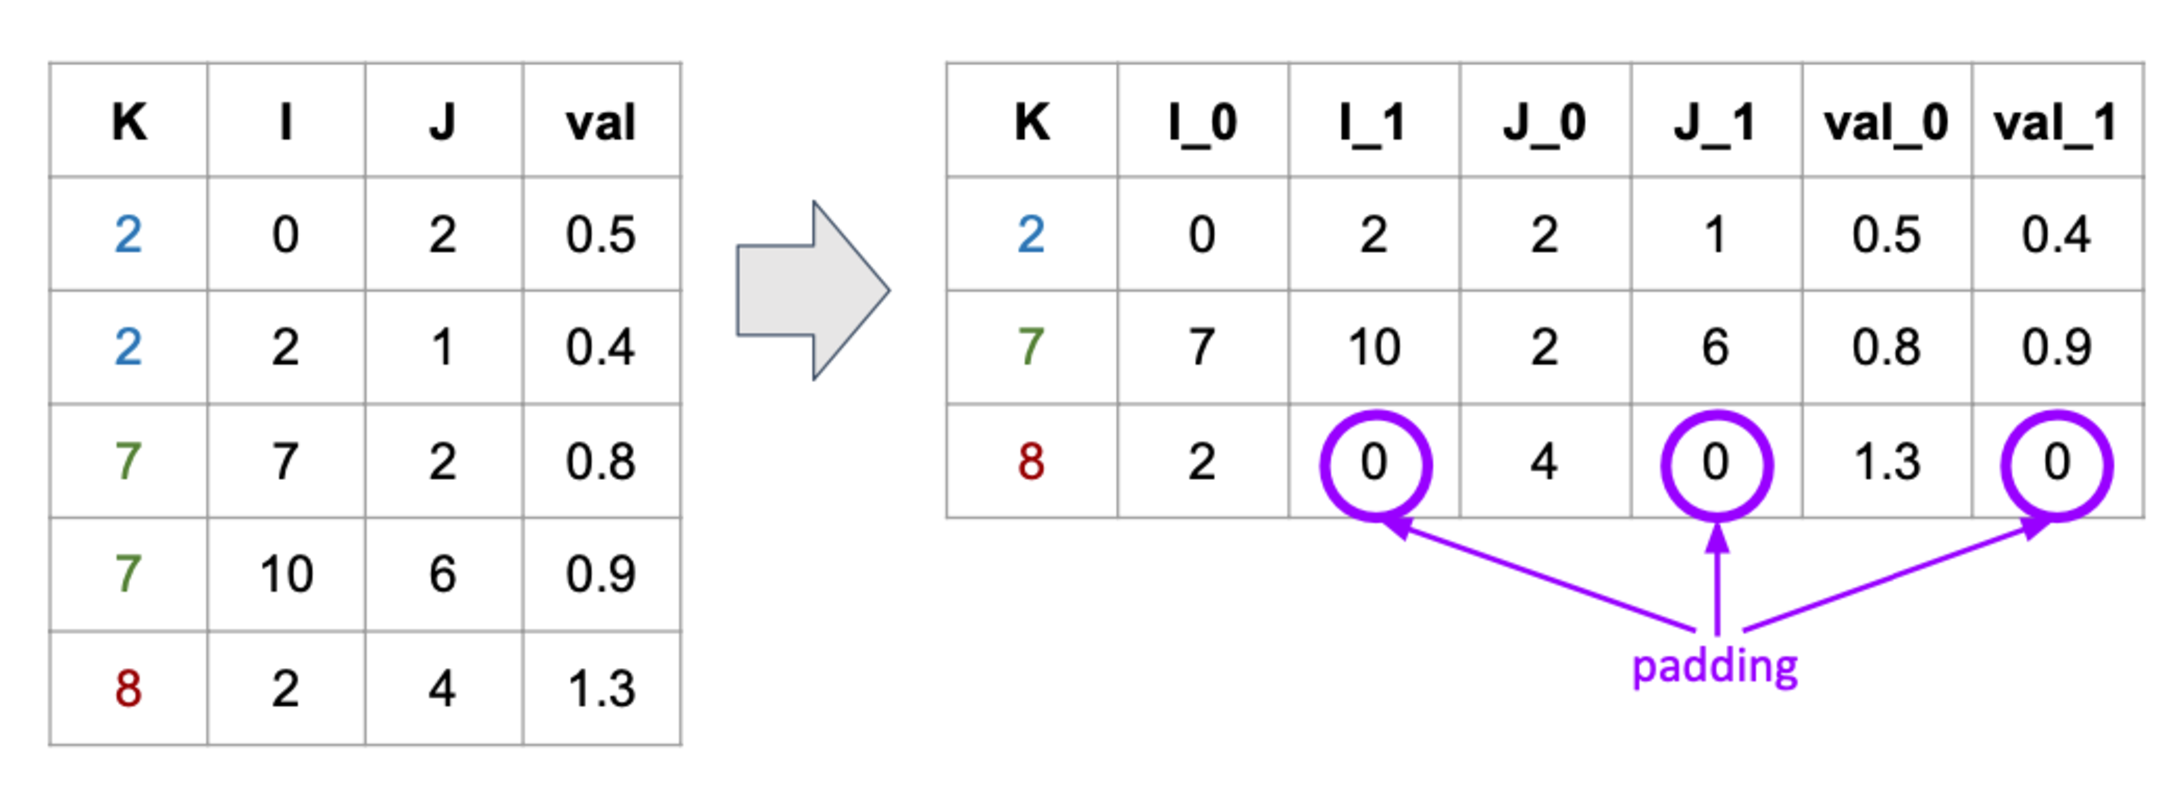
\includegraphics[width=1.0\linewidth]{grouped_coo.pdf}
  \caption{Transforming COO to a grouped COO representation with a group size of 2.}
  \label{fig:grouped_coo}
\end{figure}

An example of such grouping is shown in \autoref{fig:grouped_coo}.
We define a new parameter called a \textit{group size} which indicates how many input coordinates are grouped together for the same output coordinate.
Notice that the ideal group size varies per output coordinate,
as the number of input coordinate pairs that have the same output coordinate differ.
To make this amenable to GPUs,
we choose a single group size for all output coordinates and \textit{pad} the input coordinates'
values with zeros if they are not divisible by the group size.
For example, \autoref{fig:grouped_coo} shows that output coordinate 8 only has one input coordinate for it,
so we pad it to match the group size of 2.

%\begin{figure}[!htb]
\begin{lstlisting}[caption={Hash table lookup code.}, label={lst:improved_tensor_prod}, style=custompython]
# B : Batch size
# G_NNZ: Number of grouped output coordinates
# G: group size
# W_i, W_j, W_val: [G_NNZ, G]
# W_k: [G_NNZ]
# Input1, Input2: [B, L_in]
# Output: [B, L_out]
def TensorProduct(W_i, W_j, W_k, W_val, 
  Input1, Input2, Output):
    for nz in range(G_NNZ):
      for g in range(G)
        nz_in1 = Input1[:,W_i[nz, g]]
        nz_in2 = Input2[:,W_j[nz, g]]
        accum += nz_in1 * nz_in2 * W_val[nz, g]
      Output[:,W_k[nz]] += accum
\end{lstlisting}
%\end{figure}

The pseudocode for our improved tensor product kernel is shown in \autoref{lst:improved_tensor_prod}. Each program now loads a block of groups, where each group contains the input coordinate pairs for a given output coordinate. Because each thread now works on a single group, it can accumulate the results across that group locally before storing it back to global memory.

Because grouping introduces padded values, it increases ineffectual computation: compared to the naive implementation which performed $2NNZ \times B$ floating-point multiplies,
grouping now performs $2G\_NNZ \times G \times B$ multiplies where $G\_NNZ >= NNZ$.
The increase in work is determined by the distribution of non-zeros in the weight matrix.
As we will show in the evaluation (\autoref{sec:eval})
we sweep the group size parameter that produces the fastest runtime for our application.



\section{Evaluation}
\label{sec:eval}




%%%%%%%%% -- BIB STYLE AND FILE -- %%%%%%%%
\bibliographystyle{IEEEtranS}
\bibliography{refs,confs}
%%%%%%%%%%%%%%%%%%%%%%%%%%%%%%%%%%%%
%\begin{thebibliography}{00}
%\bibitem{b1} Tillet, Philippe, Hsiang-Tsung Kung, and David Cox. "Triton: an intermediate language and compiler for tiled neural network computations." Proceedings of the 3rd ACM SIGPLAN International Workshop on Machine Learning and Programming Languages. 2019.
%\end{thebibliography}
%\vspace{12pt}
\end{document}

